\documentclass{article}
\usepackage{graphicx} % Required for inserting images
\usepackage{polski}
\input{setup}
\usepackage[margin=2cm]{geometry}
\title{Ewolucja stanów elektronowych w podwójnej kropce kwantowej: metoda Cranka--Nicolson i~Askara--Cakmaka}
\author{Marta Wleklińska}
\date{\today}

\begin{document}

\maketitle

\section{Wstęp}
Ćwiczenie polegało na symulacji układu w podwójnej kropce kwantowej: czyli układu skończonej studni potencjału $V_1$ na długości $x \in (-\infty, -d_1)\cup (d_1, \infty)$, w której znajduje się bariera o wysokości $V_2$ przy $x\in (-d_2, d_2)$ ($d_1>d_2$).\\
\\
Problem będzie rozpatrywany w czasie, wobec tego hamiltonian zależny od czasu przyjmie postać
\begin{gather}
    \mathbf{\hat{H}}(t) = -\frac{1}{2m^*}\pdv[2]{x} + V_{\text{w}}(x) + V_{t}(x, t),
    \label{eq:hamiltonian}
\end{gather}
przy czym potencjał uwięzienia $V_{\text{w}}(x)$ będzie opisywał uwięzienie w danej studni, a zależny od czasu czynnik $V_{t}(x, t)$ opisuje wpływ pola elektrycznego dany wzorem
\begin{equation}
    V_t(x, t) = Fx\sin(\omega t).
    \label{eq:time dependent ele}
\end{equation}
\subsection{Schemat Cranka--Nicolson}
Procedura znajdowania funkcji falowej będzie podzielona na dwie części:
\begin{enumerate}
    \item \textit{Primowana} funkcja falowa $\Psi_i'$ będzie zdefiniowana jako
    \begin{gather}
        \Psi'_i = -\alpha \left(\Psi_{i+1} + \Psi_{i-1} - 2 \Psi_{i}\right) + V_{\text{w}}(x_i)\Psi_i + Fx_i\sin(\omega t)\Psi_i, \quad i = 1, 2, ... , n-2,
    \end{gather}
    przy odpowiednich funkcjach $\Psi_0, \Psi_{n-1}$.
    \item Przybliżenie funkcji $\Psi$
    \begin{gather}
        \Psi^{(k+1)} = \Psi(t_i) + \frac{\Delta t}{2\ii}\Psi^{(k)}.
    \end{gather}
\end{enumerate}
Powyższą procedurę powtarzamy dziesięciokrotnie, uzyskując $\Psi^{(k=10)} \equiv \Psi(t_1)$.
\subsection{Schemat Askara--Cakmaka}
Do opisu systemu poprzez schemat Askara--Cakmaka, użyjemy wyniku początkowego ze schematu Cranka--Nicolson.
Funkcja falowa w kolejnych krokach czasowych będzie przyjmowała postać
\begin{gather}
    \Psi(x, t_{m+1}) = \Psi(x, t_{m-1}) - {2\Delta t}{\ii}\mathbf{\hat{H}}\Psi(x, t_{m}).
\end{gather}
W symulacji w jednostkach atomowych przyjęliśmy wartość kroku czasowego \texttt{dt = 1}.


\section{Wyniki}
\subsection{Energia układu w funkcji amplitudy pola elektrycznego}
Pierwsza część ćwiczenia polegała na zdefiniowaniu systemu podwójnej studni potencjału i zbadanie układu przy hamiltonianie niezależnym od czasu
\begin{gather}
    \mathbf{\hat{H}} = -\frac{1}{2m^*}\pdv[2]{x} + V_{\text{w}}(x) + Fx.
\end{gather}
Zbudowany został zatem hamiltonian i rozwiązany problem własny, w którym mogliśmy znaleźć odpowiednie energie własne.
Pierwsze cztery energie zostały przedstawione na rysunku~\ref{fig:ex1}.
\begin{figure}[htp!]
    \centering
    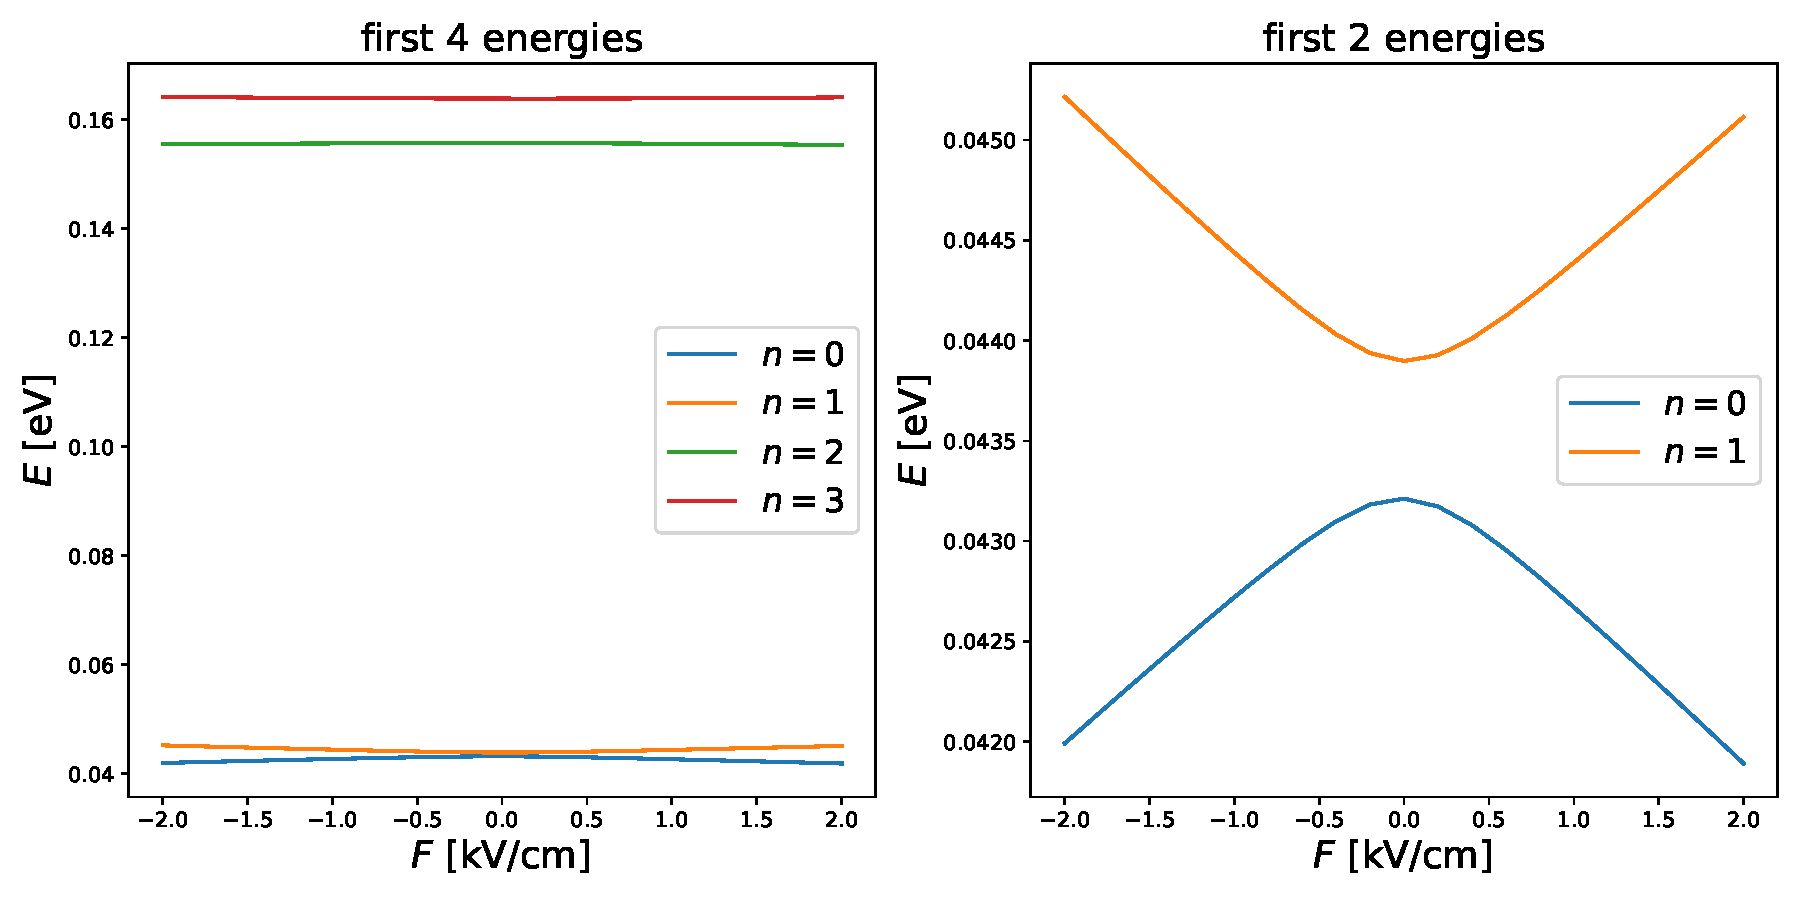
\includegraphics[width=0.9\linewidth]{ex1.pdf}
    \caption{Zależność energii od amplitudy pola elektrycznego $F$}
    \label{fig:ex1}
\end{figure}
Dodatkowo, pierwsze dwa stany zostały przedstawione w przybliżeniu.
Na pierwszej zależności od razy możemy zauważyć, że pierwsze dwie energie oraz trzecia z czwartą są zgrupowane blisko siebie.
Przybliżając jednak każde z nich możemy zauważyć, że dla stanu $n=0$ i $n=1$ energie monotonicznie zbliżają się do siebie przy $F\in [-2; 0^-)$ oraz monotonicznie oddalają się od siebie przy $F\in (0^+; 2]$.
Energie trzecia oraz czwarta są stałe w funkcji amplitudy $F$.
Porównując wyniki dwóch pierwszych energii z pozycją~\cite{Kim2015}, otrzymujemy delikatnie różniące się wyniki względem zachowania się pierwszego stanu, jako że ten przy $F\in (0^+; 2]$ - maleje, a nie rośnie, jak w naszych wynikach.
Wynika to z serii przybliżeń (1D, 1 elektron), które zostały zaimplementowane w~symulacji.

\subsection{Układ bez pola elektrycznego}
Kolejne ćwiczenie polegało na znalezieniu funkcji falowych przyjmując wartość $F = 0$.
Ponownie, procedura obejmowała zbudowanie hamiltonianiu i rozwiązanie problemu własnego, otrzymując odpowiednie wektory własne, które zostały następnie unormowane.
Wyniki kolejnych $n=0, 1$ funkcji falowych wraz z potencjałem studni zostały przedstawione na rysunku~\ref{fig:ex2}.
\begin{figure}[htp!]
    \centering
    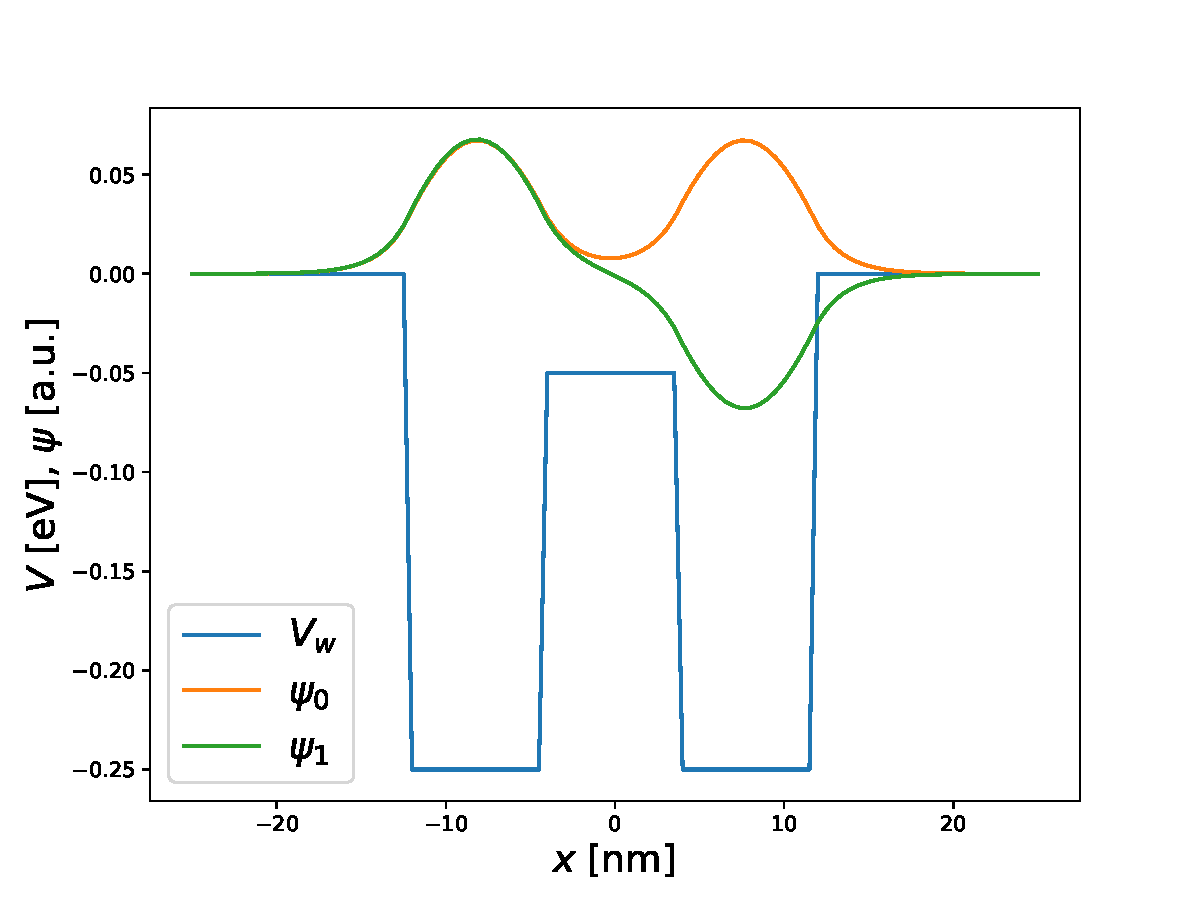
\includegraphics[width=0.75\linewidth]{ex2.pdf}
    \caption{Funkcje falowe w układzie podwójnej studni}
    \label{fig:ex2}
\end{figure}
Przy $n=0$ funkcja falowa przyjmuje niezerowe wartości dla całej dziedziny układu, podczas gdy pierwszy stan ma kształt antysymetryczny, w którym funkcja falowa w pierwszej studni przyjmuje wartości nieujemne - a w drugiej niedodatnie.

\subsection{Badanie zależności czasowej z pola elektrycznego}
Trzecia część obejmuje zbadanie układu z hamiltonianem~\eqref{eq:hamiltonian} przy potencjale pola elektrycznego~\eqref{eq:time dependent ele}.
Przyjmujemy amplitudę \texttt{F = 0.08}, krok czasowy \texttt{dt = 1.0}, \texttt{omega = 104.22e-7 * 2.418884} (wartość odpowiadająca różnicy energii między stanami) i przeprowadzamy symulację dla \texttt{3e06} kroków czasowych.
Aby przedstawić wyniki symulacji graficznie, wyznaczyliśmy kwadrat modułu rzutu funkcji falowej $\Psi (t_n)$ na stany $\ket{0}$ i $\ket{1}$.
Na rysunku~\ref{fig:ex3} pokazano prawdopodobieństwa znalezienia układu w tych stanach.
\begin{figure}[htp!]
    \centering
    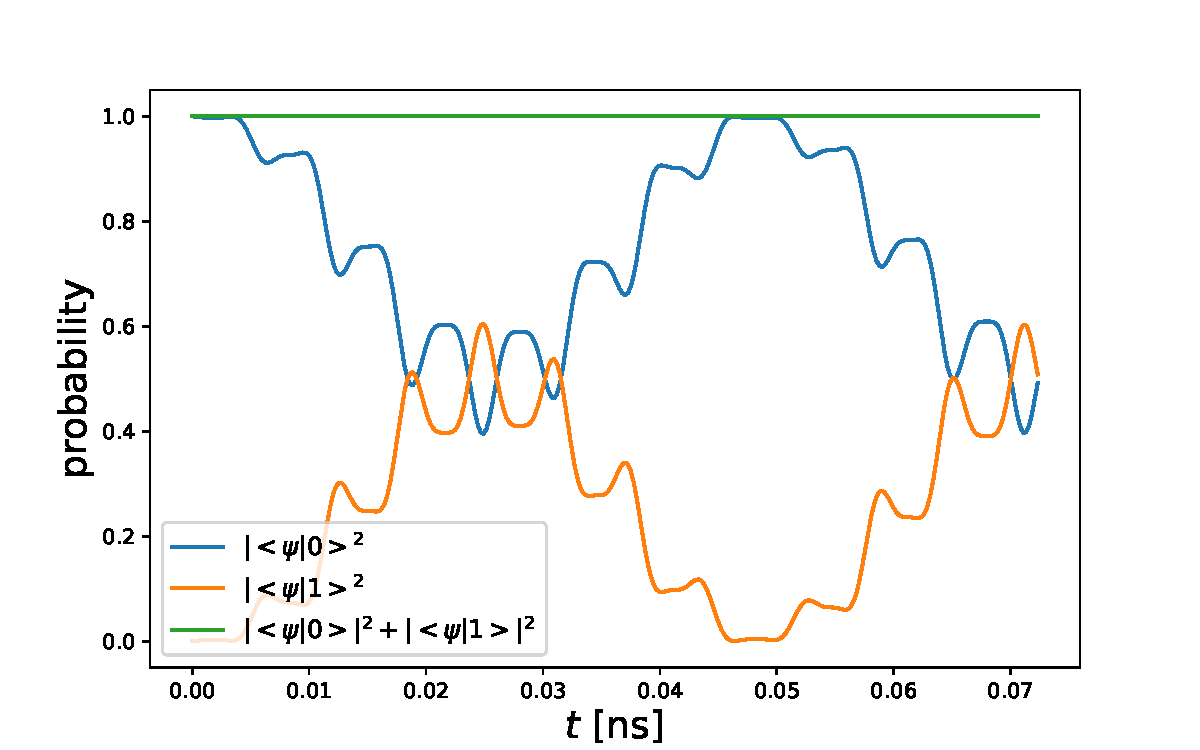
\includegraphics[width=0.8\linewidth]{ex3.pdf}
    \caption{Prawdopodobieństwa znalezienia układu w stanie $\ket{0}$ i $\ket{1}$}
    \label{fig:ex3}
\end{figure}
Wyraźnie widać sinusoidalny charakter każdej z krzywych.
Jest on jednak zaburzony w czasie — okresowo występują niewielkie spadki prawdopodobieństwa w fazie globalnego wzrostu oraz okresowe, słabe wzrosty w fazie globalnego spadku.\\
\\
Zbadano również sumę prawdopodobieństw dla obu stanów.
Wynik to stała wartość równa 1, co oznacza, że prawdopodobieństwa sumują się do całości w każdym kroku czasowym.


\section{Podsumowanie}
Ćwiczenie polegało na symulacji jednowymiarowej podwójnej kropki kwantowej.
Do opisu dynamiki układu wykorzystano metody Cranka–Nicolsona oraz Askara–Cakmaka.
Badano także wpływ pola elektrycznego — zarówno stałego, jak i zmiennego w czasie — który był uwzględniany w kolejnych wersjach hamiltonianu układu.
%%%%%%%%%%%%%%%%%
\bibliographystyle{unsrt}
\bibliography{bib}
\end{document}
